%% This is an example first chapter.  You should put chapter/appendix that you
%% write into a separate file, and add a line \include{yourfilename} to
%% main.tex, where `yourfilename.tex' is the name of the chapter/appendix file.
%% You can process specific files by typing their names in at the 
%% \files=
%% prompt when you run the file main.tex through LaTeX.

\singlespacing{

\chapter{Design Hierarchy}

Parts\\
Functions\\
Modules\\
Systems\\


\section{Parts}

At the lowest level, bulk materials in the form of \textit{parts} are assembled together to form multimaterial assemblies.  
Parts components are on the order of ~1um\textsuperscript{3}.

\section{Functions}

Assemblies of \textit{parts} form components called textit{functions}.
Functional Components are on the order of ~1mm\textsuperscript{3}.

\section{Modules}

\section{Systems}

\section{Examples}

\subsection{CA}

\begin{figure}
  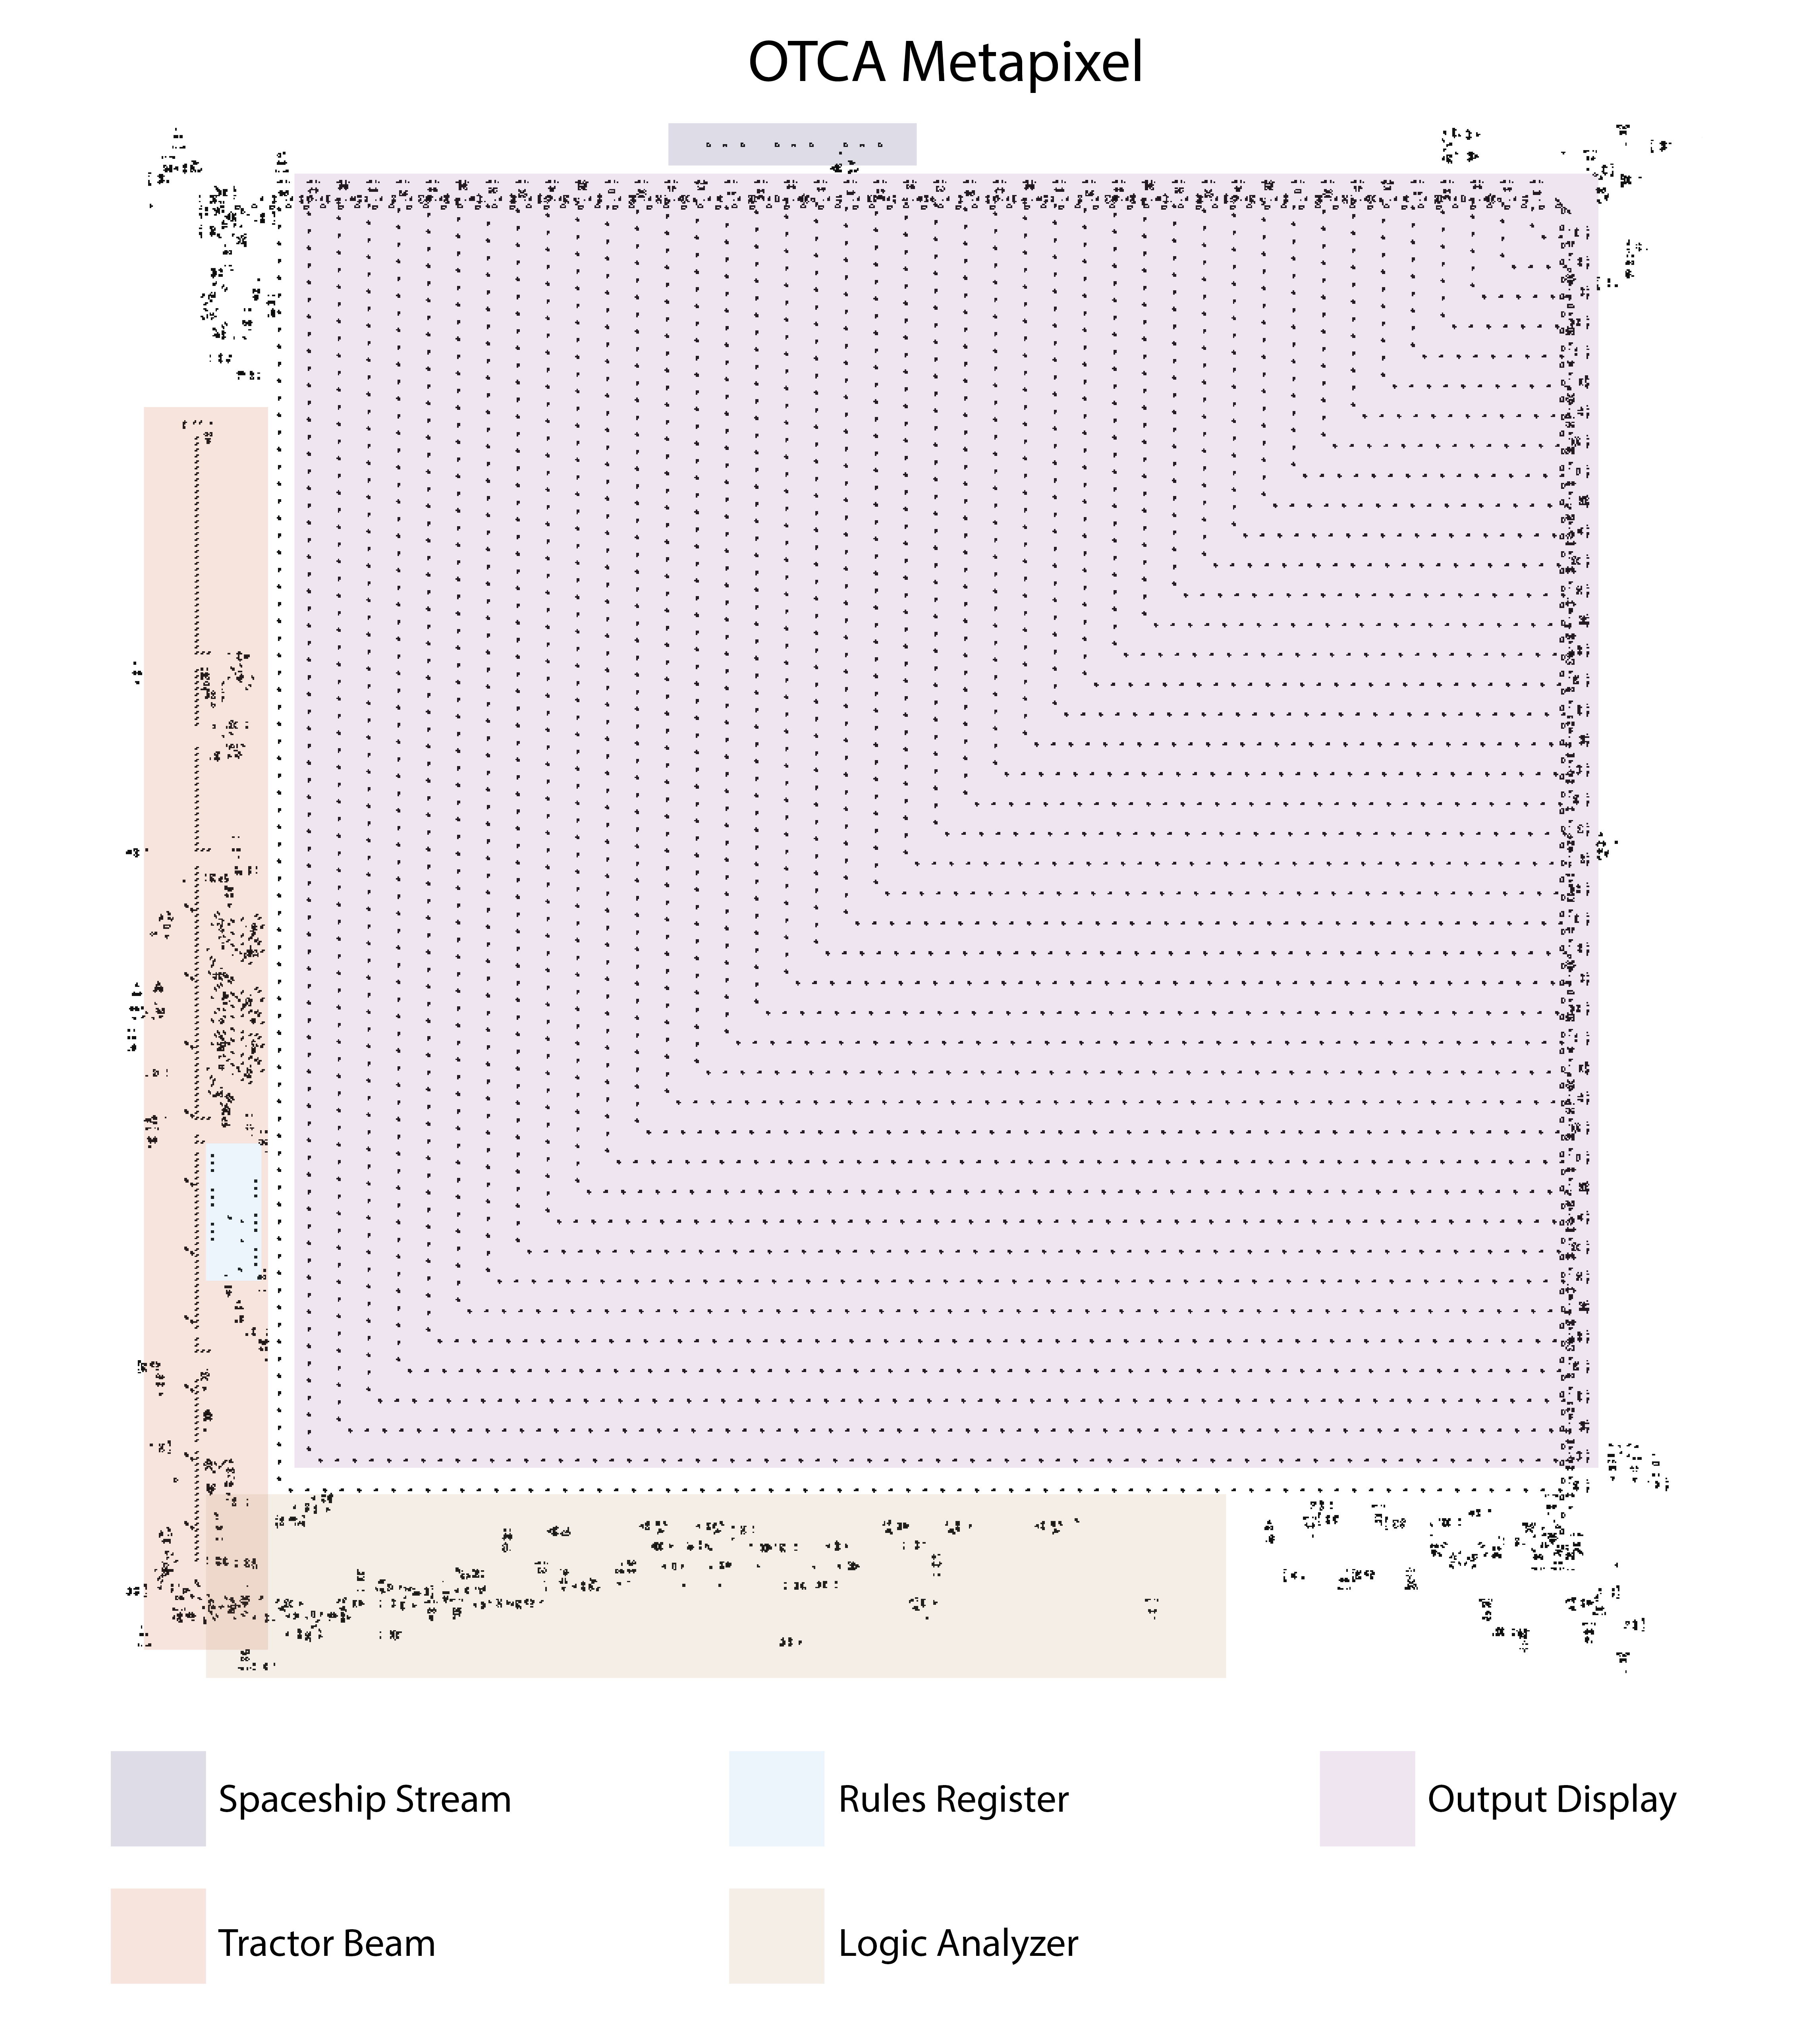
\includegraphics[width=\textwidth]{OTCADiagram.png}
  \caption{System level diagram of OTCA Metapixel with the most important modules highlighted.}
  \label{fig:OTCADiagram}
\end{figure}

\begin{sidewaysfigure}
  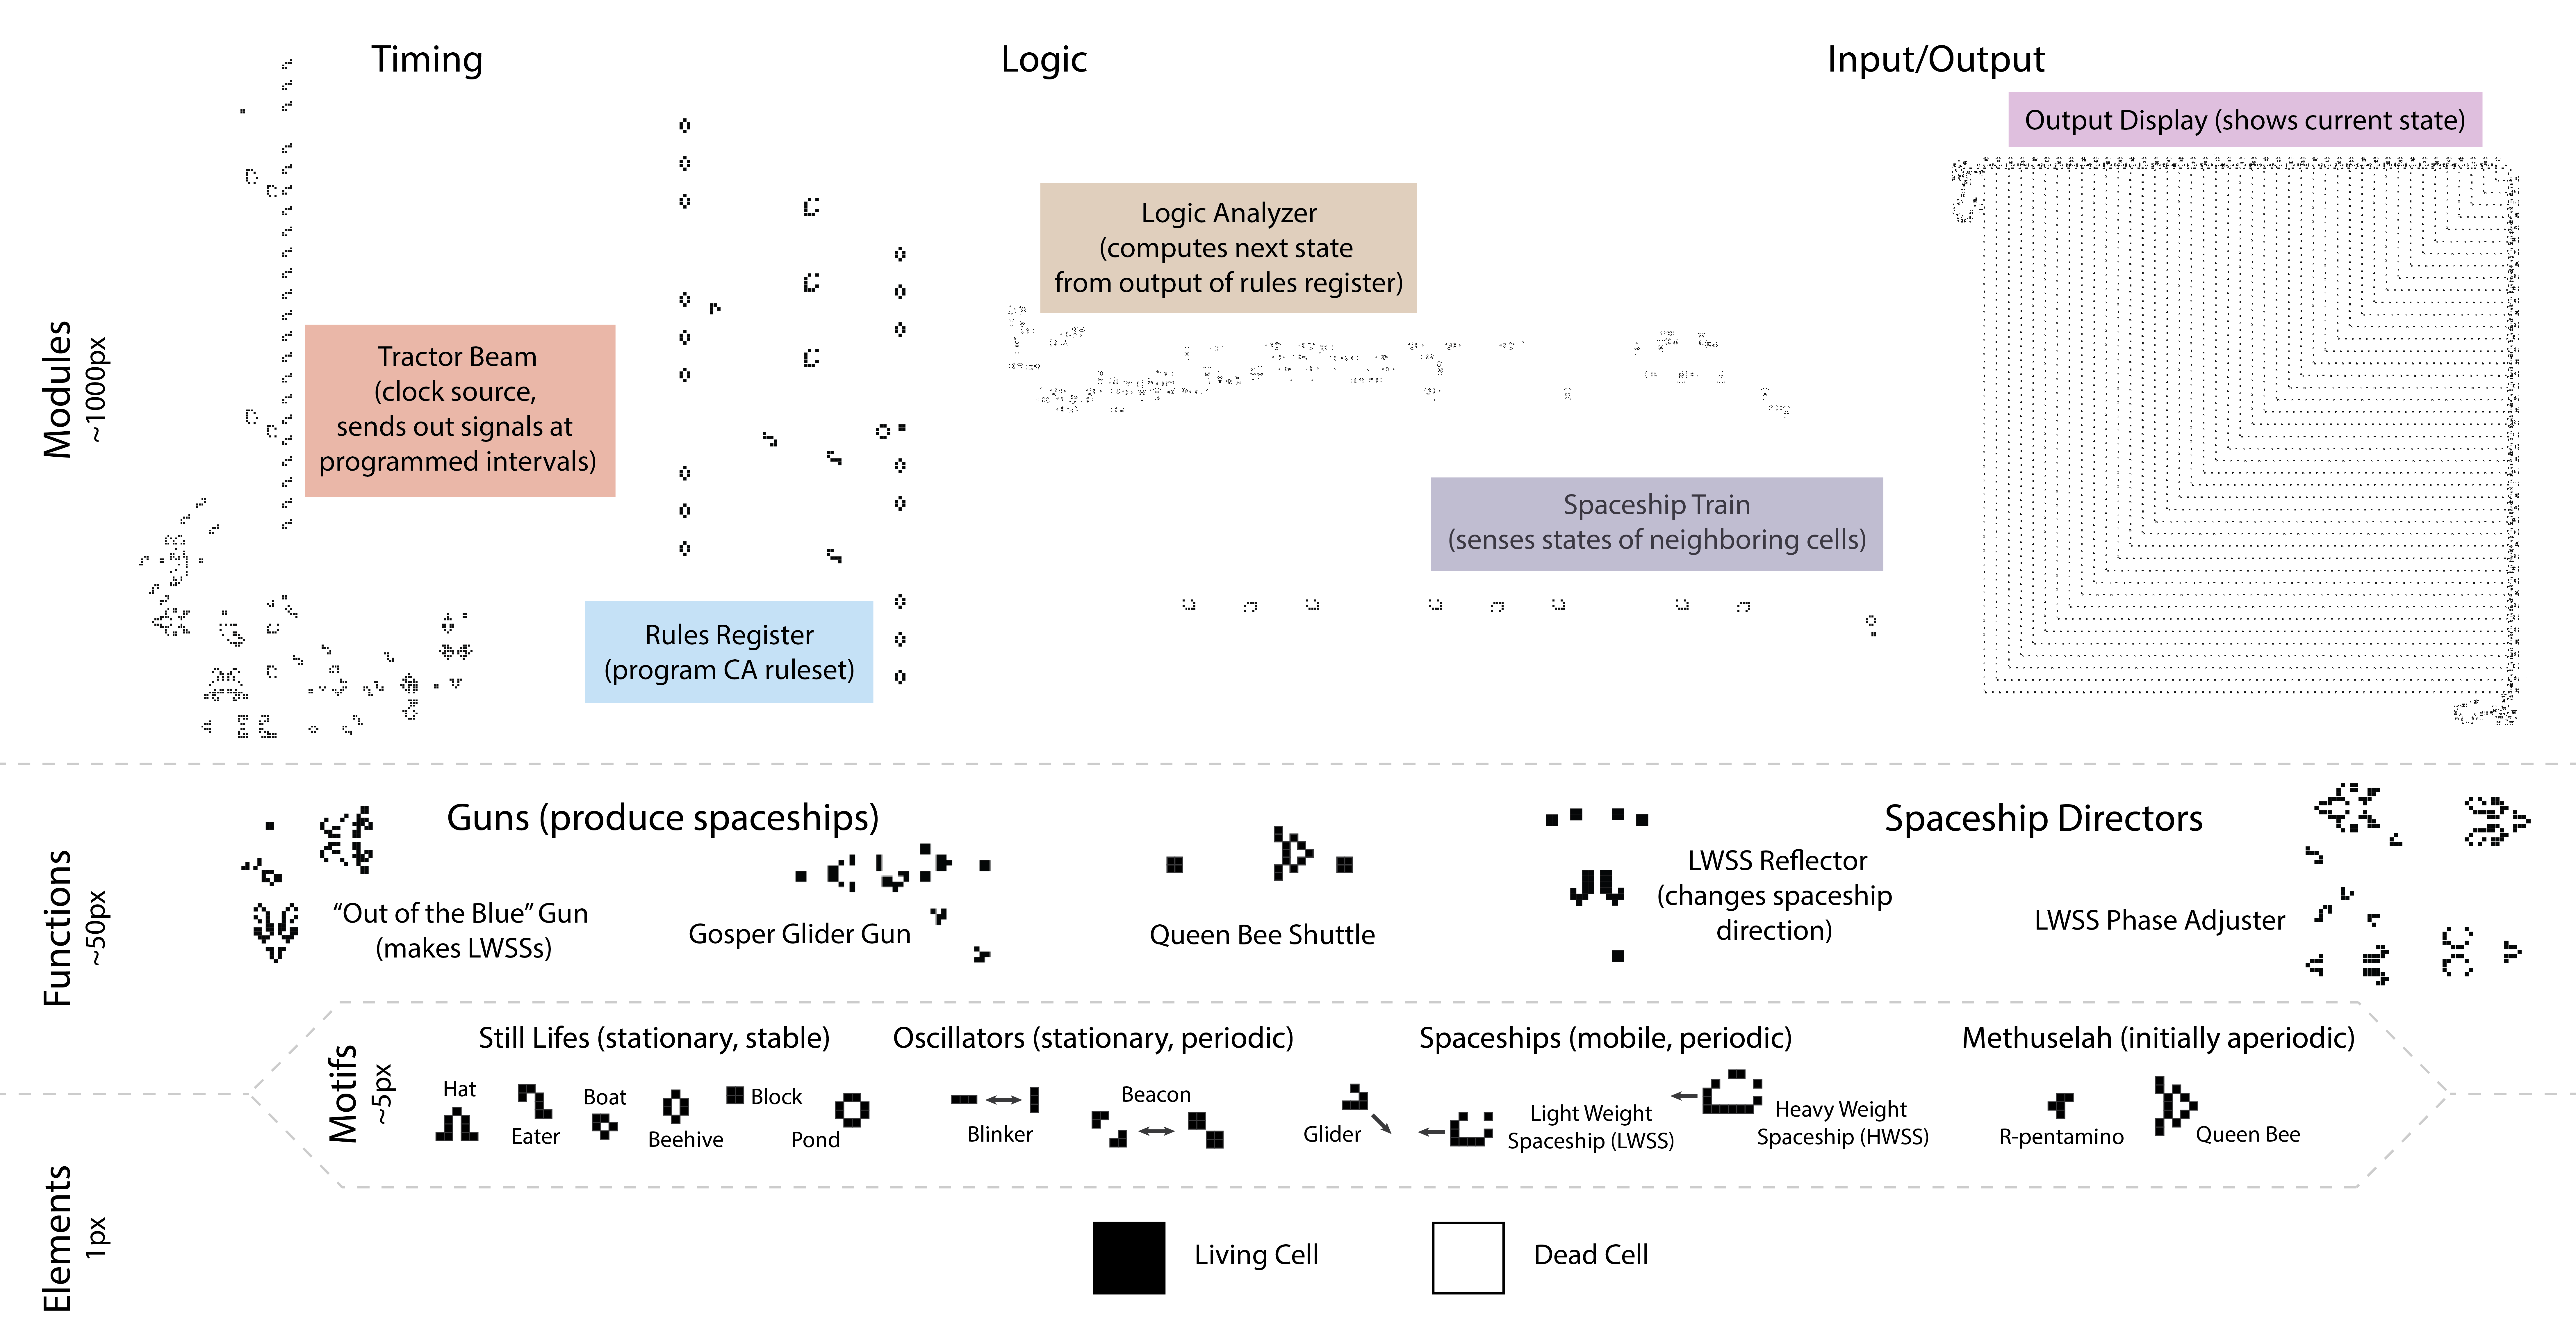
\includegraphics[width=\textwidth,height=\textheight,keepaspectratio]{OTCAMetaHierarchy.png}
  \caption{Hierarchical breakdown of OTCA Metapixel.}
  \label{fig:OTCAMetaHierarchy}
\end{sidewaysfigure}

\section{Exceptions}

scaling mismatch between the functional density of electronic and mechanical systems, offset in hierarchical setup.

\section{Hierarchy in Simulation}

increasing simulation abstraction as hierarchical level increases\\

In the next chapters, I'll describe the methods used to simulate parts and functions, and describe how abstractions of the parts-level simulation are adapted to the functions-level.



}
